% Diagrama de flujo PRISMA 2020 · RSL perturbación proactiva
% Compilable solo (pdflatex prisma_rsl.tex) o incluible en el artículo:
%   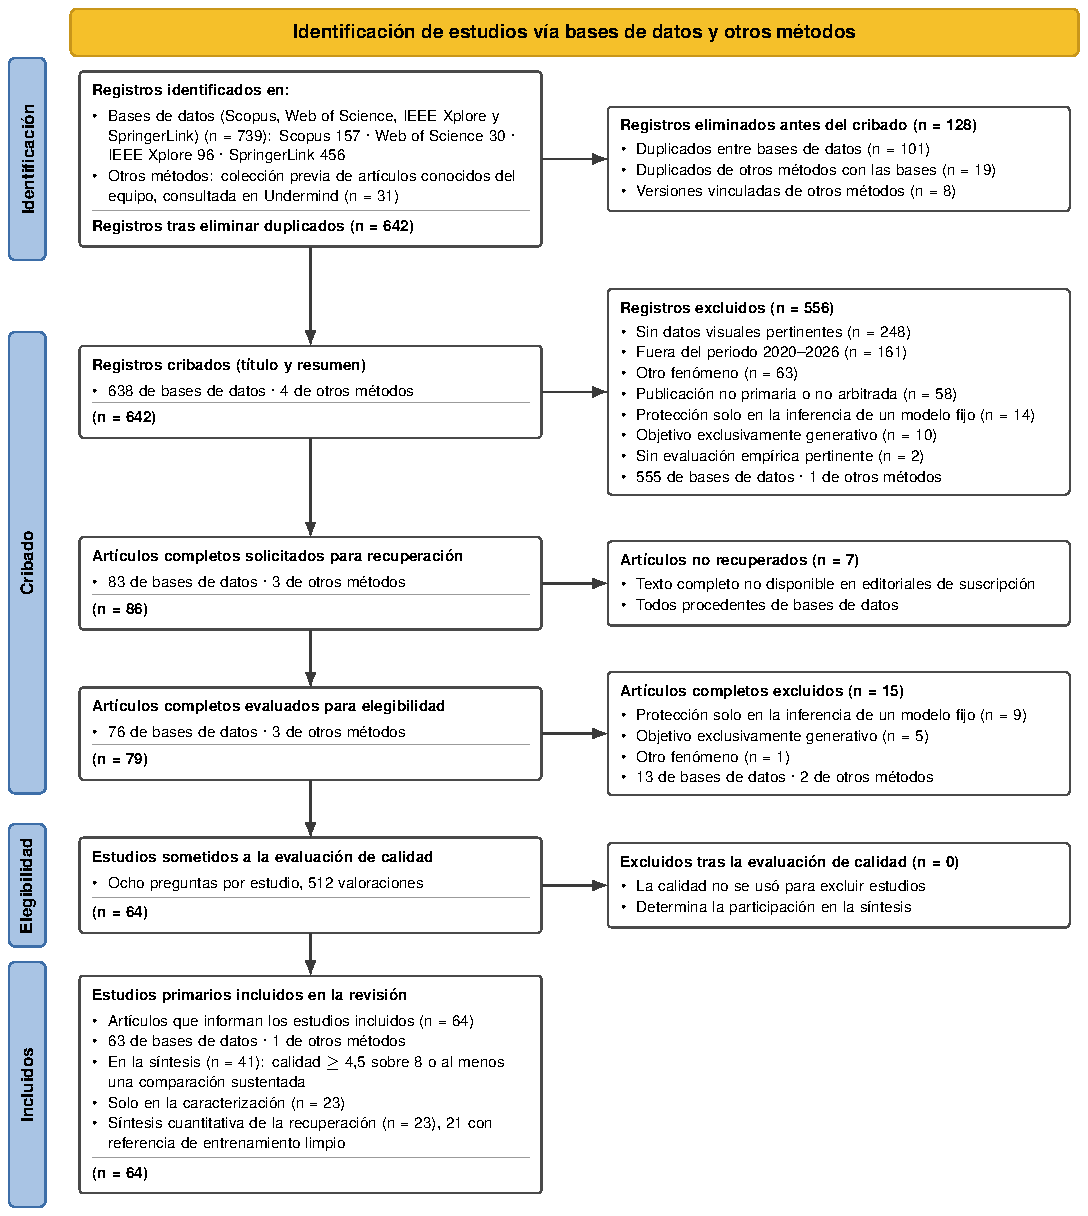
\includegraphics[width=\textwidth]{prisma_rsl.pdf}
\documentclass[border=4pt]{standalone}
\usepackage[T1]{fontenc}
\usepackage[utf8]{inputenc}
% babel no es necesario en la figura: no genera rótulos automáticos
\usepackage[scaled=0.92]{helvet}
\renewcommand{\familydefault}{\sfdefault}
\usepackage{xcolor}
\usepackage{enumitem}
\usepackage{tikz}
\usetikzlibrary{positioning,fit,matrix,calc,arrows.meta}

% ---------------------------------------------------------------- cifras
% Identificación
\newcommand{\nBases}{739}
\newcommand{\nScopus}{157}
\newcommand{\nWoS}{30}
\newcommand{\nIEEE}{96}
\newcommand{\nSpringer}{456}
\newcommand{\nOtros}{31}
\newcommand{\nEliminados}{128}
\newcommand{\nDupBases}{101}
\newcommand{\nDupOtros}{19}
\newcommand{\nVersiones}{8}
\newcommand{\nTrasDup}{642}
% Cribado
\newcommand{\nCribBases}{638}
\newcommand{\nCribOtros}{4}
\newcommand{\nExclTA}{556}
\newcommand{\nExclTABases}{555}
\newcommand{\nExclTAOtros}{1}
\newcommand{\nSolicitados}{86}
\newcommand{\nSolBases}{83}
\newcommand{\nSolOtros}{3}
\newcommand{\nNoRecup}{7}
\newcommand{\nEvaluados}{79}
\newcommand{\nEvalBases}{76}
\newcommand{\nEvalOtros}{3}
\newcommand{\nExclTC}{15}
\newcommand{\nExclTCBases}{13}
\newcommand{\nExclTCOtros}{2}
% Elegibilidad
\newcommand{\nCalidad}{64}
% Incluidos
\newcommand{\nIncluidos}{64}
\newcommand{\nIncBases}{63}
\newcommand{\nIncOtros}{1}
\newcommand{\nSintesis}{41}
\newcommand{\nCaracterizacion}{23}
\newcommand{\nNucleo}{23}
\newcommand{\nNucleoCcero}{21}

% ---------------------------------------------------------------- estilo
\definecolor{cabecera}{HTML}{F5C02A}
\definecolor{cabeceraborde}{HTML}{C9961A}
\definecolor{banda}{HTML}{A9C4E4}
\definecolor{bandaborde}{HTML}{3D6EA8}
\definecolor{borde}{HTML}{4A4A4A}
\definecolor{flecha}{HTML}{3A3A3A}

\setlist[itemize]{leftmargin=1.05em,itemsep=0.5pt,topsep=1pt,partopsep=0pt,parsep=0pt,label=\textbullet}

\newcommand{\caja}[3]{%
  \textbf{#1}\par\vspace{2pt}%
  #2\par\vspace{2pt}%
  {\color{borde!55}\hrule height 0.4pt}\vspace{4pt}%
  \textbf{#3}}
\newcommand{\salida}[2]{\textbf{#1}\par\vspace{1pt}#2}

\begin{document}
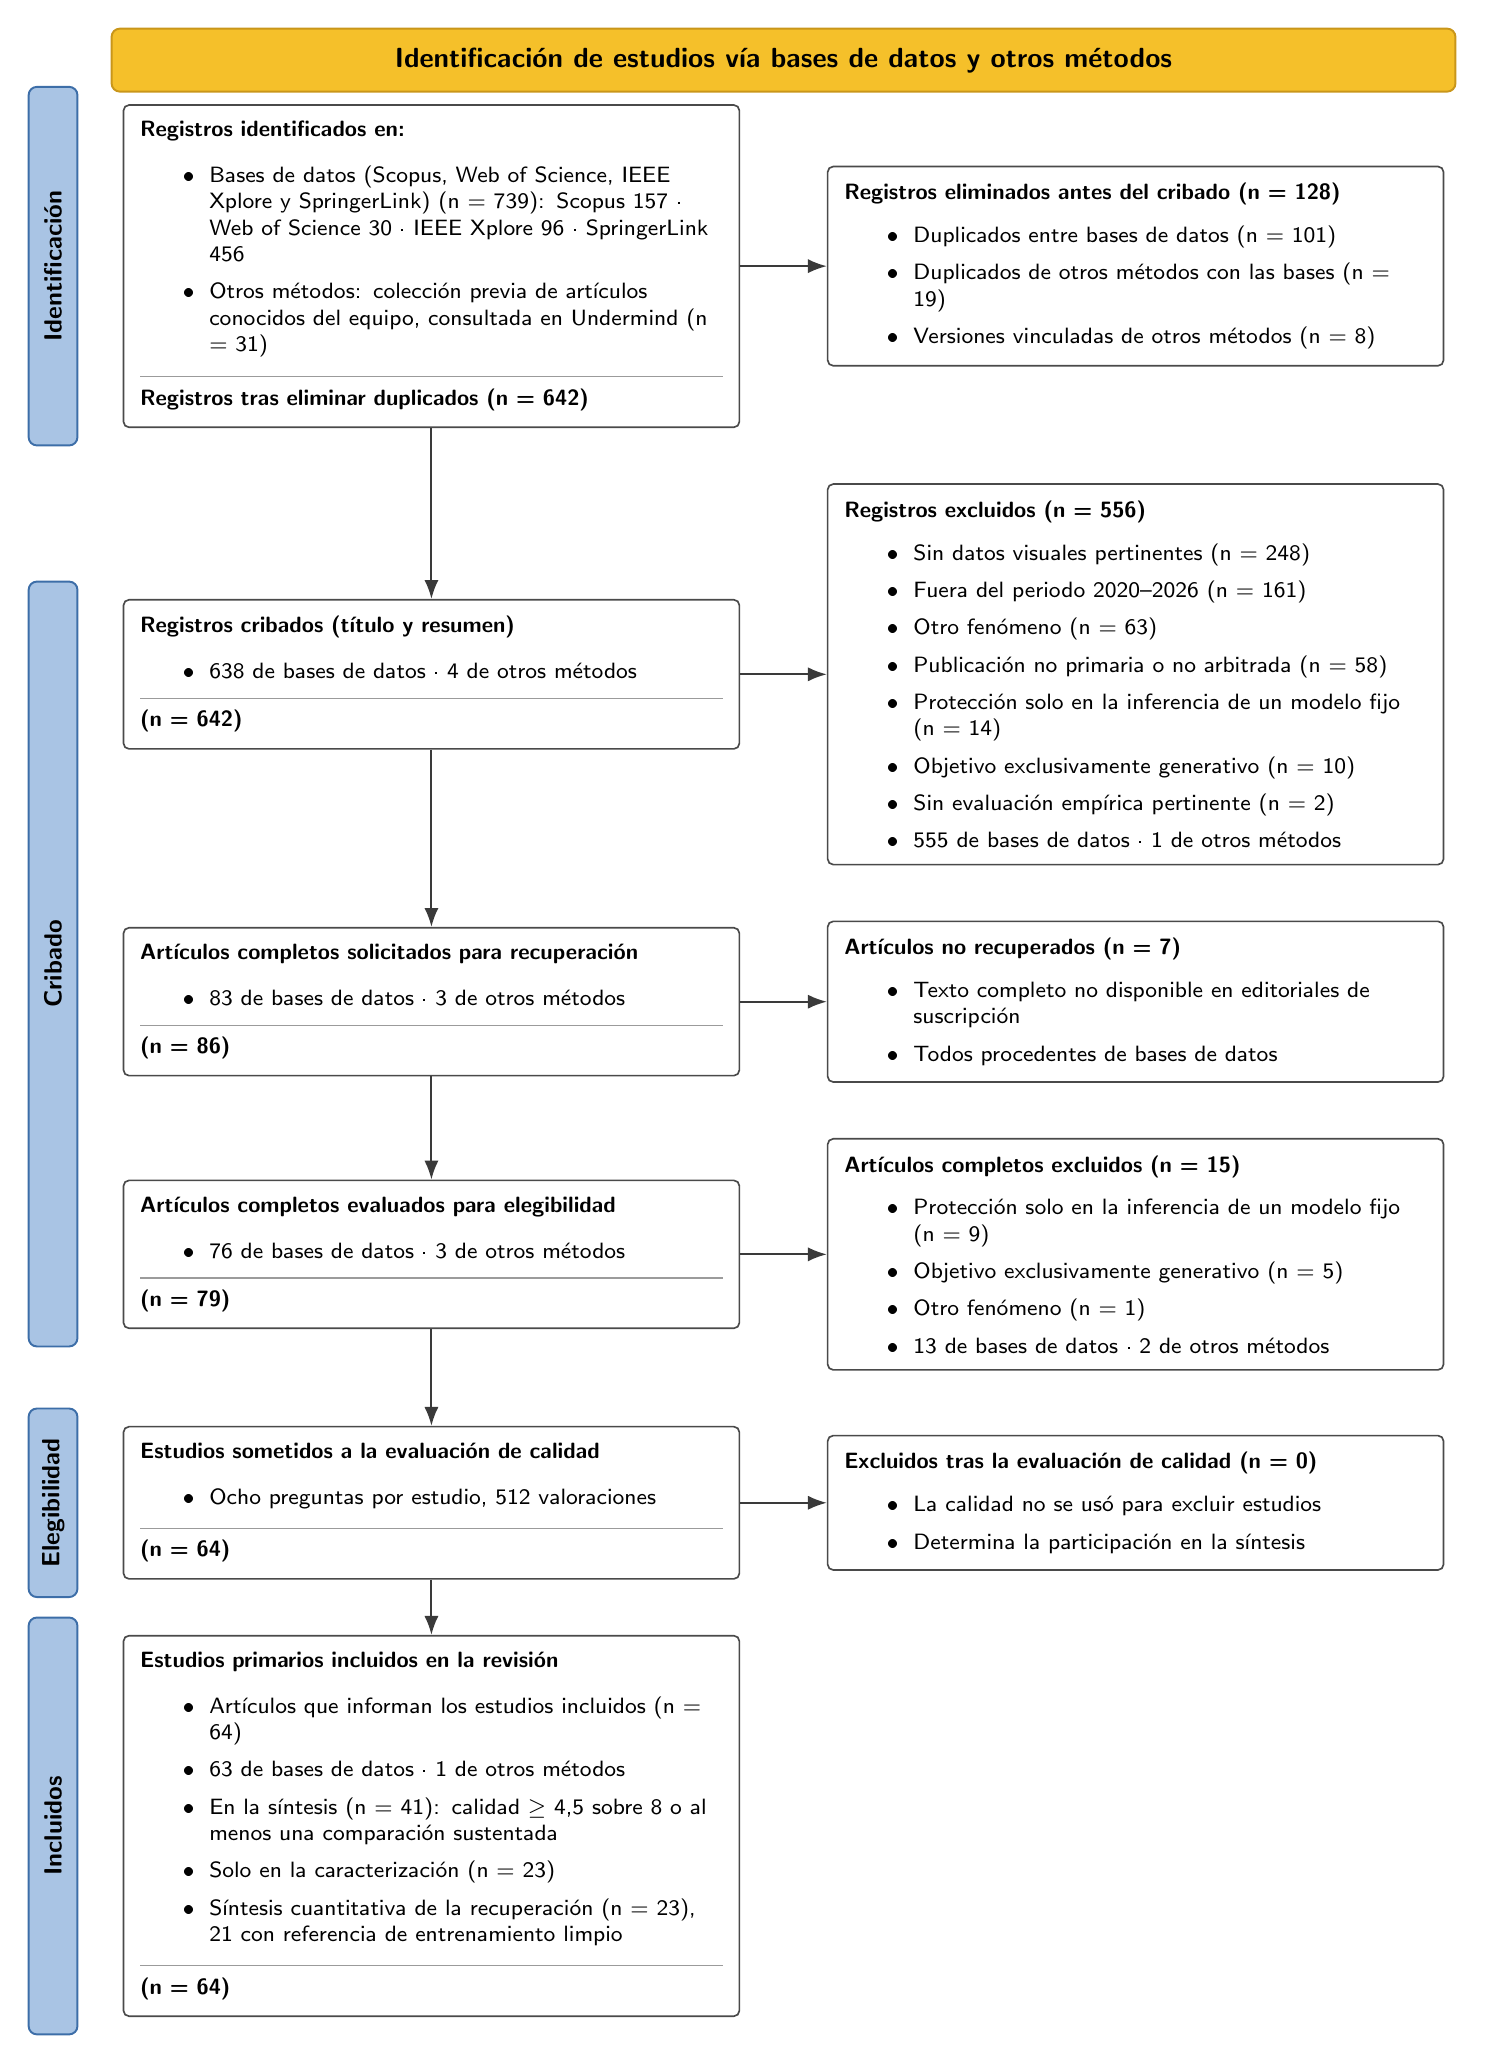
\begin{tikzpicture}[
  font=\footnotesize,
  principal/.style={draw=borde, line width=0.6pt, rounded corners=2pt, fill=white,
    text width=7.4cm, align=left, inner sep=6pt},
  lateral/.style={draw=borde, line width=0.6pt, rounded corners=2pt, fill=white,
    text width=7.4cm, align=left, inner sep=6pt},
  banda/.style={draw=bandaborde, line width=0.7pt, rounded corners=3pt, fill=banda},
  sig/.style={-{Latex[length=2.4mm,width=1.8mm]}, line width=0.7pt, draw=flecha},
]

\matrix (m) [matrix of nodes, ampersand replacement=\&, row sep=7mm, column sep=11mm,
             nodes={anchor=center}] {
% ---------------------------------------------------------------- Identificación
|[principal]| {\caja{Registros identificados en:}{%
  \begin{itemize}
  \item Bases de datos (Scopus, Web of Science, IEEE Xplore y SpringerLink)
        (n = \nBases): Scopus \nScopus{} · Web of Science \nWoS{} ·
        IEEE Xplore \nIEEE{} · SpringerLink \nSpringer
  \item Otros métodos: colección previa de artículos conocidos del equipo,
        consultada en Undermind (n = \nOtros)
  \end{itemize}}{Registros tras eliminar duplicados (n = \nTrasDup)}}
\&
|[lateral]| {\salida{Registros eliminados antes del cribado (n = \nEliminados)}{%
  \begin{itemize}
  \item Duplicados entre bases de datos (n = \nDupBases)
  \item Duplicados de otros métodos con las bases (n = \nDupOtros)
  \item Versiones vinculadas de otros métodos (n = \nVersiones)
  \end{itemize}}}
\\
% ---------------------------------------------------------------- Cribado
|[principal]| {\caja{Registros cribados (título y resumen)}{%
  \begin{itemize}
  \item \nCribBases{} de bases de datos · \nCribOtros{} de otros métodos
  \end{itemize}}{(n = \nTrasDup)}}
\&
|[lateral]| {\salida{Registros excluidos (n = \nExclTA)}{%
  \begin{itemize}
  \item Sin datos visuales pertinentes (n = 248)
  \item Fuera del periodo 2020--2026 (n = 161)
  \item Otro fenómeno (n = 63)
  \item Publicación no primaria o no arbitrada (n = 58)
  \item Protección solo en la inferencia de un modelo fijo (n = 14)
  \item Objetivo exclusivamente generativo (n = 10)
  \item Sin evaluación empírica pertinente (n = 2)
  \item \nExclTABases{} de bases de datos · \nExclTAOtros{} de otros métodos
  \end{itemize}}}
\\
|[principal]| {\caja{Artículos completos solicitados para recuperación}{%
  \begin{itemize}
  \item \nSolBases{} de bases de datos · \nSolOtros{} de otros métodos
  \end{itemize}}{(n = \nSolicitados)}}
\&
|[lateral]| {\salida{Artículos no recuperados (n = \nNoRecup)}{%
  \begin{itemize}
  \item Texto completo no disponible en editoriales de suscripción
  \item Todos procedentes de bases de datos
  \end{itemize}}}
\\
|[principal]| {\caja{Artículos completos evaluados para elegibilidad}{%
  \begin{itemize}
  \item \nEvalBases{} de bases de datos · \nEvalOtros{} de otros métodos
  \end{itemize}}{(n = \nEvaluados)}}
\&
|[lateral]| {\salida{Artículos completos excluidos (n = \nExclTC)}{%
  \begin{itemize}
  \item Protección solo en la inferencia de un modelo fijo (n = 9)
  \item Objetivo exclusivamente generativo (n = 5)
  \item Otro fenómeno (n = 1)
  \item \nExclTCBases{} de bases de datos · \nExclTCOtros{} de otros métodos
  \end{itemize}}}
\\
% ---------------------------------------------------------------- Elegibilidad
|[principal]| {\caja{Estudios sometidos a la evaluación de calidad}{%
  \begin{itemize}
  \item Ocho preguntas por estudio, 512 valoraciones
  \end{itemize}}{(n = \nCalidad)}}
\&
|[lateral]| {\salida{Excluidos tras la evaluación de calidad (n = 0)}{%
  \begin{itemize}
  \item La calidad no se usó para excluir estudios
  \item Determina la participación en la síntesis
  \end{itemize}}}
\\
% ---------------------------------------------------------------- Incluidos
|[principal]| {\caja{Estudios primarios incluidos en la revisión}{%
  \begin{itemize}
  \item Artículos que informan los estudios incluidos (n = \nIncluidos)
  \item \nIncBases{} de bases de datos · \nIncOtros{} de otros métodos
  \item En la síntesis (n = \nSintesis): calidad $\geq$ 4,5 sobre 8 o al
        menos una comparación sustentada
  \item Solo en la caracterización (n = \nCaracterizacion)
  \item Síntesis cuantitativa de la recuperación (n = \nNucleo), \nNucleoCcero{} con
        referencia de entrenamiento limpio
  \end{itemize}}{(n = \nIncluidos)}}
\&
\\
};

% ---------------------------------------------------------------- flechas
\foreach \a/\b in {1/2,2/3,3/4,4/5,5/6} {
  \draw[sig] (m-\a-1.south) -- (m-\b-1.north);
}
\foreach \r in {1,...,5} {
  \draw[sig] (m-\r-1.east) -- (m-\r-2.west);
}

% ---------------------------------------------------------------- bandas
\coordinate (bx) at ($(m.west)+(-0.45,0)$);
\newcommand{\banda}[3]{%
  \node[banda, fit={($(bx|-#1.north)+(-0.62,0.22)$) ($(bx|-#2.south)+(0,-0.22)$)}, inner sep=0pt] (b#3) {};
  \node[rotate=90, font=\small\bfseries, text=black] at (b#3) {#3};}
\banda{m-1-1}{m-1-1}{Identificación}
\banda{m-2-1}{m-4-1}{Cribado}
\banda{m-5-1}{m-5-1}{Elegibilidad}
\banda{m-6-1}{m-6-1}{Incluidos}

% ---------------------------------------------------------------- cabecera
\node[draw=cabeceraborde, line width=0.7pt, rounded corners=3pt, fill=cabecera,
      font=\normalsize\bfseries, minimum height=8mm, inner sep=4pt,
      fit={($(m-1-1.north west)+(0,0.55)$) ($(m-1-2.north east)+(0,1.35)$)}] (cab) {};
\node[font=\normalsize\bfseries] at (cab) {Identificación de estudios vía bases de datos y otros métodos};

\end{tikzpicture}
\end{document}
